\documentclass[journal]{IEEEtran}
\usepackage[a5paper, margin=10mm]{geometry}
%\usepackage{lmodern} % Ensure lmodern is loaded for pdflatex
\usepackage{tfrupee} % Include tfrupee package

%iffalse
\let\negmedspace\undefined
\let\negthickspace\undefined
\usepackage{gvv-book}
\usepackage{gvv}
\usepackage{cite}
\usepackage{amsmath,amssymb,amsfonts,amsthm}
\usepackage{algorithmic}
\usepackage{graphicx}
\usepackage{textcomp}
\usepackage{xcolor}
\usepackage{txfonts}
\usepackage{listings}
\usepackage{enumitem}
\usepackage{mathtools}
\usepackage{gensymb}
\usepackage{comment}
\usepackage[breaklinks=true]{hyperref}
\usepackage{tkz-euclide} 
\usepackage{listings}                                        
%\def\inputGnumericTable{}                                 
\usepackage[latin1]{inputenc}                                
\usepackage{color}                                            
\usepackage{array}                                            
\usepackage{longtable}                                       
\usepackage{calc}                                             
\usepackage{multirow}                                         
\usepackage{hhline}                                           
\usepackage{ifthen}                                           
\usepackage{lscape}
\usepackage{tabularx}
\usepackage{array}
\usepackage{float}
\usepackage{multicol}

\newcommand{\BEQA}{\begin{eqnarray}}
\newcommand{\EEQA}{\end{eqnarray}}
%\newcommand{\define}{\stackrel{\triangle}{=}}

\setlength{\headheight}{1cm} % Set the height of the header box
\setlength{\headsep}{0mm}     % Set the distance between the header box and the top of the text

%\usepackage[a5paper, top=10mm, bottom=10mm, left=10mm, right=10mm]{geometry}


\setlength{\intextsep}{10pt} % Space between text and floats

% Marks the beginning of the document
\begin{document}
\onecolumn
\bibliographystyle{IEEEtran}
\vspace{3cm}

%\renewcommand{\theequation}{\theenumi}
\numberwithin{equation}{section}
\numberwithin{figure}{section}
% \renewcommand{\thefigure}{\theenumi}
\renewcommand{\thetable}{\theenumi}

\title{8.4.24}
\author{AI24BTECH11031 - Shivram S}
\maketitle

% \renewcommand{\thefigure}{\theenumi}
\renewcommand{\thetable}{\theenumi} 

\setcounter{section}{1}
\textbf{Question: } The altitude of a right-angled triangle is 7 cm less than its base. If the
hypotenuse if 13 cm, find the other two sides.
\bigskip

\textbf{Solution: } 

\begin{table}[h!]    
	\centering
	\begin{tabular}[12pt]{ |c| c| c|}
    \hline
    \textbf{Variable} & \textbf{Description} & \textbf{Value}\\
	\hline
	$C_1$ & Equation of first conic & $x^2 + x + 12 = y$\\
	\hline
	$C_2$ & Equation of second conic & $x^2 + y^2 = 4$\\
	\hline
\end{tabular}
	\caption{Variables Used}
\end{table}

Let the length of the base be $x$ cm. The altitude of the triangle is 7 cm less than its base, i.e.,
$x - 7$ cm. By Pythagoras' Theorem
\begin{align}
    AB^2 + AC^2 = BC^2 \\
    x^2 + (x - 7)^2 = 13^2 \\
    2x^2 - 14x - 120 = 0 \\
    x^2 - 7x - 60 = 0 \\
\end{align}
The equation $y = x^2 - 7x - 60$ can be expressed as a conic
\begin{align}
    \vec{x}^\top\vec{V}\vec{x} + 2\vec{u}^\top\vec{x} + f = 0 \\
    \vec{V} = \myvec{1 & 0 \\ 0 & 0}, \vec{u} = \myvec{-\frac{7}{2} \\ -\frac{1}{2}}, f = -60
\end{align}
To find the roots of the equation, we find the points of intersection of the 
conic with the $x$-axis
\begin{align}
    \vec{x} = \vec{h} + k\vec{m} \\
    \vec{h} = \myvec{0 \\ 0}, \vec{m} = \myvec{1 \\ 0}
\end{align}
The values of $k$ are given by
\begin{align}
    k_i &= \frac{1}{\vec{m}^\top\vec{V}\vec{m}}\brak{-\vec{m}^\top\brak{\vec{V\vec{h} + \vec{u}}} \pm \sqrt{
        \sbrak{\vec{m}^\top\brak{\vec{V}\vec{h} + \vec{u}}}^2 - g\brak{\vec{h}}\brak{\vec{m}^\top\vec{V}\vec{m}}
    }} \\
    &= \frac{1}{1} \brak{\frac{7}{2} \pm \sqrt{\brak{\frac{7}{2}}^2 + 60}} \\
    k_1 &= -5, k_1 = 12
\end{align}
Hence the points of intersection are
\begin{align}
    \vec{h} + k\vec{m} = \myvec{-5 \\ 0}, \myvec{12 \\ 0}
\end{align}

Hence the solutions of the equation are $x = -5$ and $x = 12$. We reject $x = -5$ as the length of the side
can't be negative. Hence, the lengths of the sides are
\begin{align}
    AB = 12\ cm \\
    AC = 7\ cm \\
    BC = 13\ cm
\end{align}

\begin{figure}[h!]
    \centering
    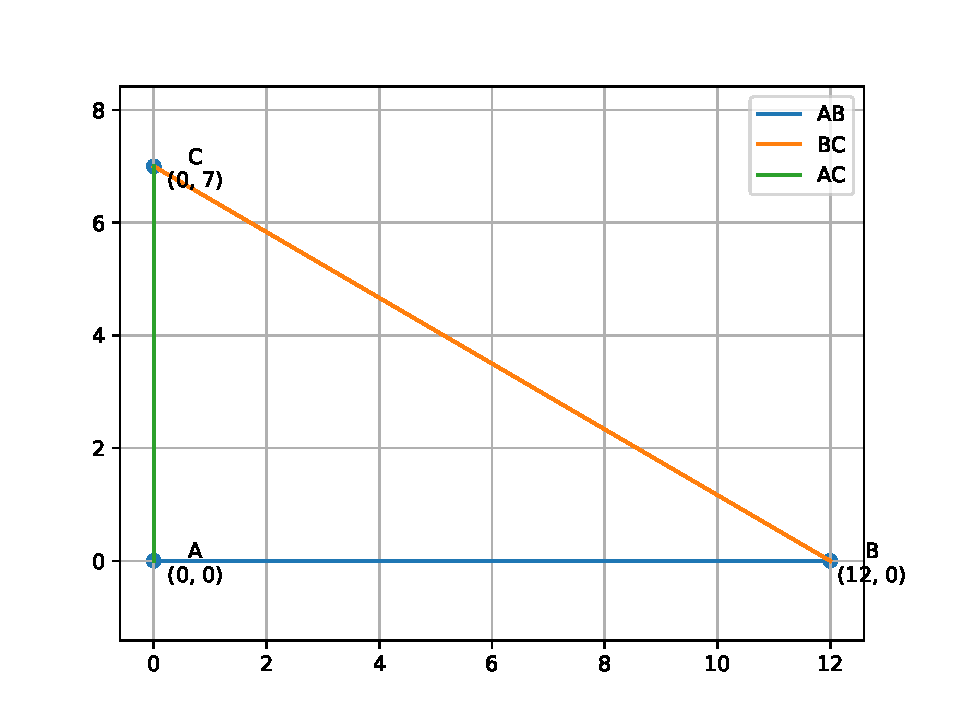
\includegraphics[width=0.7\linewidth]{figs/fig.pdf}
    \caption{Triangle with sides $AB = 12$ cm, $AC = 7$ cm, and $BC = 13$ cm}
\end{figure}
\end{document}
